% !TeX encoding=utf8
% !TeX spellcheck=de-DE

\documentclass[
  draft=false,     % draft mode (no images, layout errors shown)
  paper=a4,
  paper=portrait,
  parskip=half,    % Full empty line between paragraphs
  %   parindent=0pt,
  pagesize=auto,   % driver
  fontsize=12pt,
  version=last,    % KOMA Script version
  %   twoside,
  ]{scrartcl}

  % Encoding of _files and directories_
  % (ensures that any file can be loaded without problems)
  \usepackage[%
  extendedchars, encoding, multidot, space,
  filenameencoding=latin1, % Windows XP, Vista, 7
  % filenameencoding=utf8,   % Linux, OS X
]{grffile}

% ~~~~~~~~~~~~~~~~~~~~~~~~~~~~~~~~~~~~~~~~~~~~~~~~~~~~~~~~~~~~~~~~~~~~~~~~
% preamble
% ~~~~~~~~~~~~~~~~~~~~~~~~~~~~~~~~~~~~~~~~~~~~~~~~~~~~~~~~~~~~~~~~~~~~~~~~

%% select/load fonts
% !TeX encoding=utf8
% !TeX spellcheck = en-US

\usepackage{cmap}           % Make PDF files searchable and copyable 

\usepackage[T1]{fontenc}    % Font encoding

\usepackage{textcomp}       % Additional Symbols (Text Companion font extension)

%\usepackage{lmodern}        % LaTeX standard font
\usepackage{charter}        % Charter font
\usepackage[nosfdefault]{sourcesanspro}
\usepackage[nottdefault]{sourcecodepro}

%\usepackage{fontspec-luatex}

%\setmainfont[
%    Path           = Charter,
%    Extension      = .otf,
%    Ligatures      = TeX,
%    BoldFont       = Charter Bold,
%    ItalicFont     = Charter Italic,
%    BoldItalicFont = Charter Bold Italic
%]{Charter Regular}
%% load packages
% !TeX encoding=utf8
% !TeX spellcheck = en-US
% !TeX root=../UID_Project_Documentation.tex

%% Base packages

\usepackage{calc}	        % Calculation

\usepackage[                % Multi language support
    main=ngerman,
%    british,                % For the european date format in the bibliographies
%    ngerman,
]{babel}

\usepackage[utf8]{inputenc} % UTF-8 text encoding

\usepackage[		        % Color support with color mixing models
    dvipsnames, % Load a set of predefined colors
    table,      % Load the colortbl package
    % fixpdftex,  % Load the pdfcolmk package (may be problematic)
    hyperref,   % Support  the  hyperref  package
    fixinclude, % Prevent dvips color reset before .eps file inclusion
]{xcolor}

\usepackage[		        % Support for graphics in LaTeX
    %final,
%    draft 		% do not include images (faster)
]{graphicx}

\usepackage{wrapfig} % for wrapping text around figures

\usepackage{epstopdf}   % If an eps image is detected, epstopdf is
                        % automatically called to convert it to pdf format.

% \usepackage{ragged2e}	% environments for setting ragged text
						% which allow hyphenation.

%% Bugfixes

%\usepackage{marginnote} % marginnote allows a margin note, where \marginpar
%                        % fails
%
\usepackage{scrhack}    % Redefines implementations of
%                        % packages float, hyperref and listings
%
%\usepackage{marginfix}  % changes the \marginpar commands, such
%                        % that long margin notes work.
%
%\RequirePackage{xspace} %  Used to define commands that don't eat spaces.
%
%\usepackage[xspace]{ellipsis}   % fixes bug in ellipsis (...)

%% Fonts

\usepackage{relsize}    % Set the font size relative to the current font size

%% Math

\usepackage[            % basic math package
    centertags, % (default) center tags vertically
    %tbtags,    % 'Top-or-bottom tags': For a split equation, place equation
    % numbers level with the last (resp. first) line, if numbers
    % are on the right (resp. left).
    sumlimits,  %(default) Place the subscripts and superscripts of summation
    % symbols above and below
    %nosumlimits, % Always place the subscripts and superscripts of
    % summation-type symbols to the side, even in displayed
    % equations.
    intlimits,  % Like sumlimits, but for integral symbols.
    %nointlimits, % (default) Opposite of intlimits.
    namelimits, % (default) Like sumlimits, but for certain 'operator names'
    % such as det, inf, lim, max, min, that traditionally have
    % subscripts placed underneath when they occur in a displayed
    % equation.
    %nonamelimits, % Opposite of namelimits.
    %leqno,     % Place equation numbers on the left.
    %reqno,     % Place equation numbers on the right.
    fleqn,      % Position equations at a fixed indent from the left margin
    % rather than centered in the text column.
]{amsmath}

%\usepackage[fixamsmath,disallowspaces]{mathtools}   % The mathtools package is
%                                                    % an extension package to
%                                                    % amsmath. Furthermore it
%                                                    % corrects various bugs
%
%\usepackage[            % Inhibits the usage of plain TeX and of standard
%%LaTeX
%                        % math environments
%    all,
%    % warning
%    error
%]{onlyamsmath}
%
%\usepackage{braket}     % Macros for Dirac bra-ket notation and sets.
%
%\usepackage{cancel}     % strike out arguments in math mode
%
%\usepackage{empheq}     % Emphasize equations
%
%\usepackage{exscale}    % scales math mode output in all environments correct
%
%\usepackage{fixmath}    % fixes for the default Computer Modern math fonts
%
%\usepackage{icomma}     % Enables the correct use of the comma as a decimal
%                        % separator in math mode
%
%\usepackage{xfrac}      % LaTeX 3 Package for nice inline fractions
%                        % Provides: \sfrac{1}{2}
%
%%% Science
%
%\usepackage{siunitx}    % siunitx aims to provide a unified method to
%                        % typeset numbers and units correctly and easily.

%% Symbols

\usepackage[gen]{eurosym}   % European currency symbol

\usepackage{pifont}         % Common symbols

%% Tables

%\usepackage{booktabs}           % some additional commands to enhance the
%                                % quality of tables
%
%\usepackage{multirow, bigstrut} % extends the standard tabular environment
%%with
%                                % cells spanning over multiple rows.
%
%
%\usepackage{ltxtable}           % Table spanning over many pages (from
%                                % longtable package) and with strechable
%                                % columns (from tabularx package)
%
\usepackage{tabu}       % defines a single environment tabu to make all kinds
%                        % of tabulars. It is more flexible than tabular,
%                        % tabular*, tabularx and array and extends the
%                        % possibilities.
%
%\usepackage{tablestyles}

%% Text

% - Text decoration

\usepackage[normalem]{ulem} % commands for underlining for emphasis

\usepackage{soulutf8}       % commands for for emphasis

\usepackage{url}            % enable linebreaks for URLs

\usepackage{setspace}       % for custom line sapcing

\usepackage{float}          % better control over float environments

\usepackage[
    activate={true, compatibility},
    final,tracking=true,
%    kerning=true,
%    spacing=true,
    factor=1100,
    stretch=10
    ,shrink=10
]{microtype}

\microtypecontext{spacing=nonfrench}

% activate={true,nocompatibility} - activate protrusion and expansion
% final - enable microtype; use "draft" to disable
% tracking=true, kerning=true, spacing=true - activate these techniques
% factor=1100 - add 10% to the protrusion amount (default is 1000)
% stretch=10, shrink=10 - reduce stretchability/shrinkability (default is 20/20)

% - Footnotes

\usepackage[                % The footmisc package provides several different
%                            % customisations of the way foonotes are
%                            % represented. Fixes a LaTeX bug with option
%                            % 'bottom'
%    bottom,      % Footnotes appear always on bottom. This is necessary
%                 % especially when floats are used
%    stable,      % Make footnotes stable in section titles
    perpage,     % Reset on each page
%    %para,       % Place footnotes side by side of in one paragraph.
%    %side,       % Place footnotes in the margin
%    ragged,      % Use RaggedRight
%    %norule,     % suppress rule above footnotes
    multiple,    % rearrange multiple footnotes intelligent in the text.
%    %symbol,     % use symbols instead of numbers
]{footmisc}

% - Code listings

\usepackage{listings}

% - Quotes

\usepackage[
    autostyle,
    % german=guillemets
    ]{csquotes}

%% Bibiliography
\usepackage[
    backend=biber,
%    style=alphabetic,
    style=authoryear,
    maxcitenames=2,
%    citestyle=authortitle,
%    sorting=none
]{biblatex}

% - Abbreviations and Acronyms
\usepackage[
    acronym,
    toc
]{glossaries}
%\usepackage[
%    printonlyused,
%    withpage
%]{acronym}

% - Table of contents
\usepackage[nottoc]{tocbibind}

% - Manipulating Counters
\usepackage{chngcntr}

% - Prevent floats from going over sections
\usepackage[section]{placeins}

% - better titles
% \usepackage{titlesec}
% \newcommand{\sectionbreak}{\clearpage}

%% apply style settings
% !TeX encoding=utf8
% !TeX spellcheck = en-US

\usepackage[
    top=2.5cm,
    bottom=2cm,
    left=4cm,           % 3.5 + 0.5 Bindingoffset
    right=2.5cm,
    headheight=5ex,     % ~ 5 small x'es on top of each other
    headsep=1.25cm-\headheight, % pagetop to header = 1.25cm
    footskip=0.75cm,
]{geometry} 

\usepackage[
    autooneside=false,
    footsepline,
    plainfootsepline,
    headsepline,
    plainheadsepline,
    automark,
]{scrlayer-scrpage}

\cfoot[]{}                      % Center part of footer empty
\chead[]{}                      % Center part of footer empty
\ofoot[\pagemark]{\pagemark}    % Outer footer pagemark 
                                % (-number)						
\ohead{\rightmark}				% Outer header chapter
% -- hyphenation --
% !TeX encoding=utf8
% !TeX spellcheck = de-DE

\hyphenation{Krosch-wald}

\graphicspath{{images/}}

% Hyperref
\usepackage[
  hyperfootnotes=false
]{hyperref}

\hypersetup{
    %    colorlinks=true,    % For PDF
    %    filecolor=magenta,
    %    linkcolor=black,
    %    citecolor=black,
    %    urlcolor=blue,
    colorlinks=true,  % For Print
    filecolor=black,
    linkcolor=black,
    citecolor=black,
    urlcolor=black,
    %    linktocpage=true,
    linktoc=all,
    pdfpagelayout=OneColumn,
    pdfpagemode=UseOutlines,
%    pdfauthor=\me,
%    pdftitle=\mytitle,
    pdfdisplaydoctitle=true,
    pdfremotestartview=Fit, % Set the startup page view of remote PDF files
    pdfcenterwindow=false,
    pdffitwindow=false,     % resize document window to fit document size
    pdfnewwindow=false,
    pdfstartpage=1,
    pdfstartview=FitV,
    bookmarksopen=true,
    bookmarksnumbered=true,
    bookmarkstype=toc,
    bookmarksopenlevel=2,
}

% !TeX encoding=utf8
% !TeX spellcheck = en-US

\title{\mytitle}
\author{\me}

\newcommand{\dsh}{~--~}

\newlength{\currentparskip}
\newenvironment{minipageparskip}
{\setlength{\currentparskip}{\parskip}% save the value
    \begin{minipage}{\textwidth}% open the minipage
        \setlength{\parskip}{\currentparskip}% restore the value
    }
{\end{minipage}}

\begin{document}
    	% -- title page --
%    % !TeX encoding=utf8
% !TeX spellcheck=de-DE
% !TeX root=../UID_Project_Documentation.tex

\begin{titlepage}
   \pagestyle{empty}
   \centering
   
\includegraphics[width=\textwidth]{dhbw-karlsruhe_logo}\qquad
  % 	\includegraphics[width=6cm]{images/SAP_grad_R_pref.png}\\
   \mbox{}\vspace{4\baselineskip}\\
   \rmfamily\Large
   \centering
   Usability und User Interface Design
  % 	\vspace{1\baselineskip}
   \vspace{1\baselineskip}\\
   \sffamily\huge
   \centering
   Projektdokumentation - MyNewsApp
   \vspace{1\baselineskip}\\
   \rmfamily
   % \Large
   % Projektdokumentation - MyNewsApp\\
   \normalsize
   WWI16B1
   \vspace{1\baselineskip}\\
   
   Stefan Bergmann Alexander Gebhardt\\
   Kevin Sieverding Maximilian Stefanac\\
   Fabian Wallisch
   \vspace{3\baselineskip}\\

   6. April 2018

   % \sffamily\normalsize
   % \begin{tabular}{ll}
   %   Verfasser/in:						& \me{}\\
   %   Kurs: 								& WWI16B1\\
   %   Partnerunternehmen: 				& SAP SE\\
   %   Wissenschaftliche/r Betreuer/in: 	& Prof. Dr. Katja Wengler\\
   %   Abgabedatum: 						& 05.01.2018\\
   % \end{tabular}

\end{titlepage}


     \title{MyNewsApp: Projektdokumentation}
     \author{Stefan Bergmann \and Alexander Gebhardt \and Kevin Sieverding \and Maximilian Stefanac \and Fabian Wallisch}

     \maketitle
     \thispagestyle{empty}

     \newpage

    \pagenumbering{Roman}
    \pagestyle{plain.scrheadings}
%    \setcounter{page}{2}

     % -- table of contents --
    \microtypesetup{protrusion=false} % Disable protrusion for lists

    \tableofcontents

    \newpage

    \listoffigures

    \clearpage

    \microtypesetup{protrusion=true} % Disable protrusion for lists

    %% Content formatting

    \pagenumbering{arabic}
    \pagestyle{scrheadings}
    \setcounter{page}{1}
    \onehalfspacing{}

    % !TeX encoding=utf8
% !TeX spellcheck=de-DE
% !TeX root=../UID_Project_Documentation.tex

\section{Motivation}

\subsection{Einordnung und Problemstellung}

Das von uns erdachte Produkt beschäftigt sich mit Problemen, die beim Anbieten und Konsumieren von ehemaligen Print-Inhalten im digitalen Zeitalter entstehen und die wir als von den bisherigen Angeboten ungelöst sehen.

Mit dem Einzug von digitalen Gerätschaften und dem Internet in die Haushalte und den Alltag eines großen Teils der Weltbevölkerung ist die Nachfrage nach digitalen Inhalten jedweder Form stark und stetig gestiegen. Auch der Journalismus ist von dieser Entwicklung nicht verschont geblieben und es wird seitdem versucht sich entsprechend anzupassen. Zum Beispiel war bereits am 25. Oktober 1994 mit \enquote{Spiegel Online} eine von Deutschlands bekanntesten Quellen für Journalismus über das Netz erreichbar. Heute vertreibt praktisch jede professionelle Publikation ihre Inhalte zumindest teilweise über einen Webauftritt und muss sich dabei nicht nur gegenüber der traditionellen Konkurrenz sondern auch einer schier unzählige Masse an privaten und halb-professionellen \enquote{Bloggern} behaupten.

Diese neuen Gefilde zeigen einige Dynamiken und Aspekte auf, die sich von denen der traditionellen Vertriebswelt für Journalismus stark unterscheiden. Der moderne Nutzer ist es gewohnt alle Inhalte die er wünscht direkt abrufbar zu haben. Es ist normal verschiedenste Quellen zu konsumieren, um entweder ihre Inhalte zu einem bestimmten Thema zu vergleichen oder vielmehr sie den Schwerpunkten ihrer Kompetenz gerecht zu nutzen um sich so eine persönliche, optimierte Konsumlandschaft zu kreieren.

Durch dieses Konsumverhalten zusammen mit der stärkeren Konkurrenz an diesem transparenteren Markt, sowie den technischen Limitationen des Mediums, stellt sich das Monetarisieren von digitalen Inhalten als eine nicht zu unterschätzende Herausforderung dar.

Das einzige Geschäftsmodell, welches sich bisher wirklich durchgesetzt hat ist die Monetarisierung durch das Schalten von Werbeanzeigen. Dieses bringt allerdings einige Problemen mit sich. Durch dieses Modell wird die Wirtschaftlichkeit eines Inhalts ausschließlich durch die von ihm generierte Anzahl an Aufrufen bestimmt. Dadurch wird der Konsument der Inhalte vom Kunden der Publikationen zu deren Produkt, welches diese an die Werbeschaltenden verkaufen. Dadurch rückt der eigentliche Kunde aus dem Fokus und die Tatsache dass Werbeanzeigen generell als störend empfunden werden, wird hingenommen. Tendenziell belohnt das Modell Quantität mehr als Qualität und dadurch kurze, Aufmerksamkeit heischende Beiträge mehr als fundierte, differenzierte Berichterstattung. Vor allem aber, rechnet es sich erst ab einer hohen absoluten Zahl von Aufrufen und ist auch dann oft nicht ausreichend. Zum Beispiel erwirtschaftet die international erfolgreiche, britische Publikation \enquote{The Guardian} seit Jahren nur Verluste und muss sich durch andere Publikationen querfinanzieren.

Hieraus ergibt sich eine Situation, welche sowohl für den Konsumenten als auch für den Produzenten der Inhalte unvorteilhaft ist und wir wurden das Gefühl nicht los, dass es doch eine bessere Lösung geben muss.

\subsection{Konzept}

Wir wollten eine Lösung gestalten, die dem Nutzer all die Freiheit und Flexibilität gibt, die er von einem modernen Dienst gewohnt ist und erwartet, jedoch auch für die Anbieter von Inhalten eine effektive und faire Form der Monetarisierung darstellt. Das ganze sollte abgerundet werden durch eine intuitive und leichte Nutzererfahrung, welche die Hürden für das Verwenden unseres Dienstes und das Konsumieren von monetarisierten Inhalten durch ihn so weit wie möglich senkt.

Hierfür haben wir eine Nachrichten App entworfen, welche Inhalte von Verschiedensten Quellen auf einer möglichst granularen Ebene bereitstellt. Das bedeutet, dass man grundsätzlich für jeden Inhalt einzeln bezahlen kann oder aber auch bestimmte Sammlungen von Inhalten abonnieren kann. In der Praxis könnte man so das \enquote{Sport}-Segment von Zeitung A abonnieren, sowie alle Artikel die von Autor P geschrieben werden, die Komplette Zeitung B, als auch vereinzelte Artikel von den Zeitschriften C, D und E. Wir versuchen so die Vorteile von On-Demand- sowie Flatrate-Modellen zu nutzen. Ein Nutzer kann sich die von ihr gekauften oder abonnierten Inhalte dann in sogenannten Feeds zusammenstellen und so ihren Konsum stark personalisieren.

Bisherige Produkte, welche ehemals Print-Inhalte digital anbieten, haben zwar einige der beschriebenen Probleme gelöst indem sie ihren Kunden einen Single-Point-of-Access (SPA) für die Inhalte mehrerer Publikationen sowie die damit zusammenhängenden Transaktionen bieten. Allerdings, haben sie nicht den revolutionären Schritt getan die Struktur der Angebotenen Inhalte aufzubrechen und den Nutzern somit umfangreiche Personalisierungsmöglichkeiten beim Konsum als auch Flexibilität beim Kauf zu ermöglichen. Deswegen sind wir überzeugt, dass sich unser Produkt in dem Oligopol der digitalen Nachrichten-Plattformen gegen die Konkurrenz behaupten kann.

Während wir in dieser Ausarbeitung nur die Umsetzung unseres Konzepts als Mobile-App ausführen, so wären in einem realen Szenario jedoch auch eine Webapp, sowie angepasste Anwendungen für alle anderen gängigen Systeme Teil der Umsetzung. Hierbei würde man sich um ein möglichst eingängiges Design bemühen um Nutzern ein möglichst uniformes Erlebnis zu ermöglichen, sowie von Vertrautheit und Wiedererkennungswert zu profitieren.

    \include{content/20-Oservation}
    % !TeX encoding=utf8
% !TeX spellcheck=de-DE
% !TeX root=../UID_Project_Documentation.tex

\section{Ideation}

Bei den Sketches haben wir uns grundlegend überlegt, wie die App die Anforderungen der potenziellen Nutzer, die durch unsere Personas repräsentiert werden, gelöst werden könnten. Ein wichtiger Punkt dabei ist es den Spagat zwischen der unterschiedlichen Technikaffinität der Personas zu bedienen. Beispielsweise sollen so wenig wie möglich Kognitionsfehler bei den Nutzern entstehen und auch bei erfahrenen Nutzern so wenig wie möglich Routinefehler. Die Sketches stellen Lösungen für die Probleme der Personas dar, die in die Prototyping Phase des UCD Prozess einfließen, um den Prototypen zu gestalten. Eine weitere Herausforderung einer News-App ist, dass sehr viel Inhalt auf übersichtliche Art und Weise auf sehr begrenztem Platz untergebracht werden muss.

\subsection{Sketch 1}

\begin{figure}[h]
  \centering
  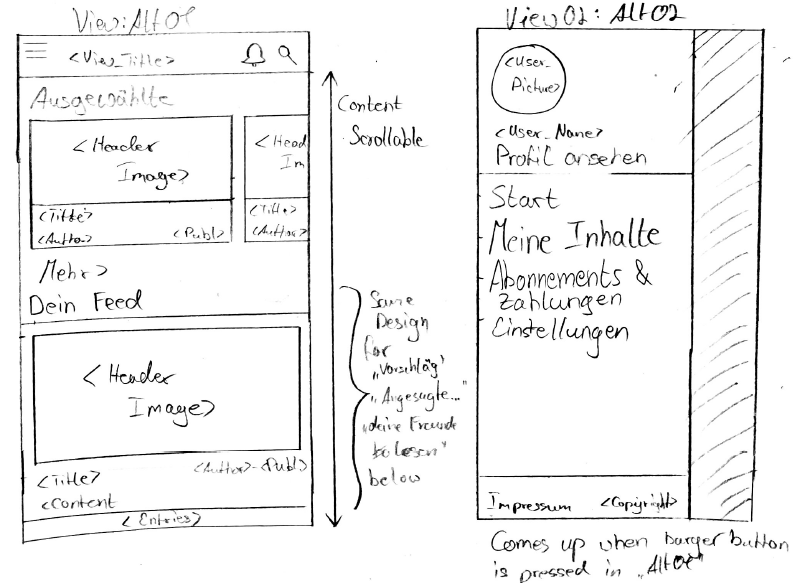
\includegraphics[width=\textwidth]{sketches 01}
  \caption{Sketch 1}
  \label{fig:sketch-01}
\end{figure}

Dieser Sketch verbindet Funktionsumfang und Übersichtlichkeit in hohem Maße, sodass daraus ein gesamtheitlich schlankes, aber intuitives Bedienkonzept resultiert. Besonders hervorzuheben ist aber der dargestellte Homescreen, sowie der Aufbau des Burgermenüs, an denen wir uns für den Prototypen orientieren möchten. Auf dem Homescreen befinden sich so verschiedene Gruppen von Artikeln, wie zum Beispiel \enquote{dein Feed} oder \enquote{Ausgewählte}, die es ermöglichen, eine Mehrzahl an Artikeln logisch strukturiert darzustellen.

\subsection{Sketch 2}

\begin{figure}[h]
  \centering
  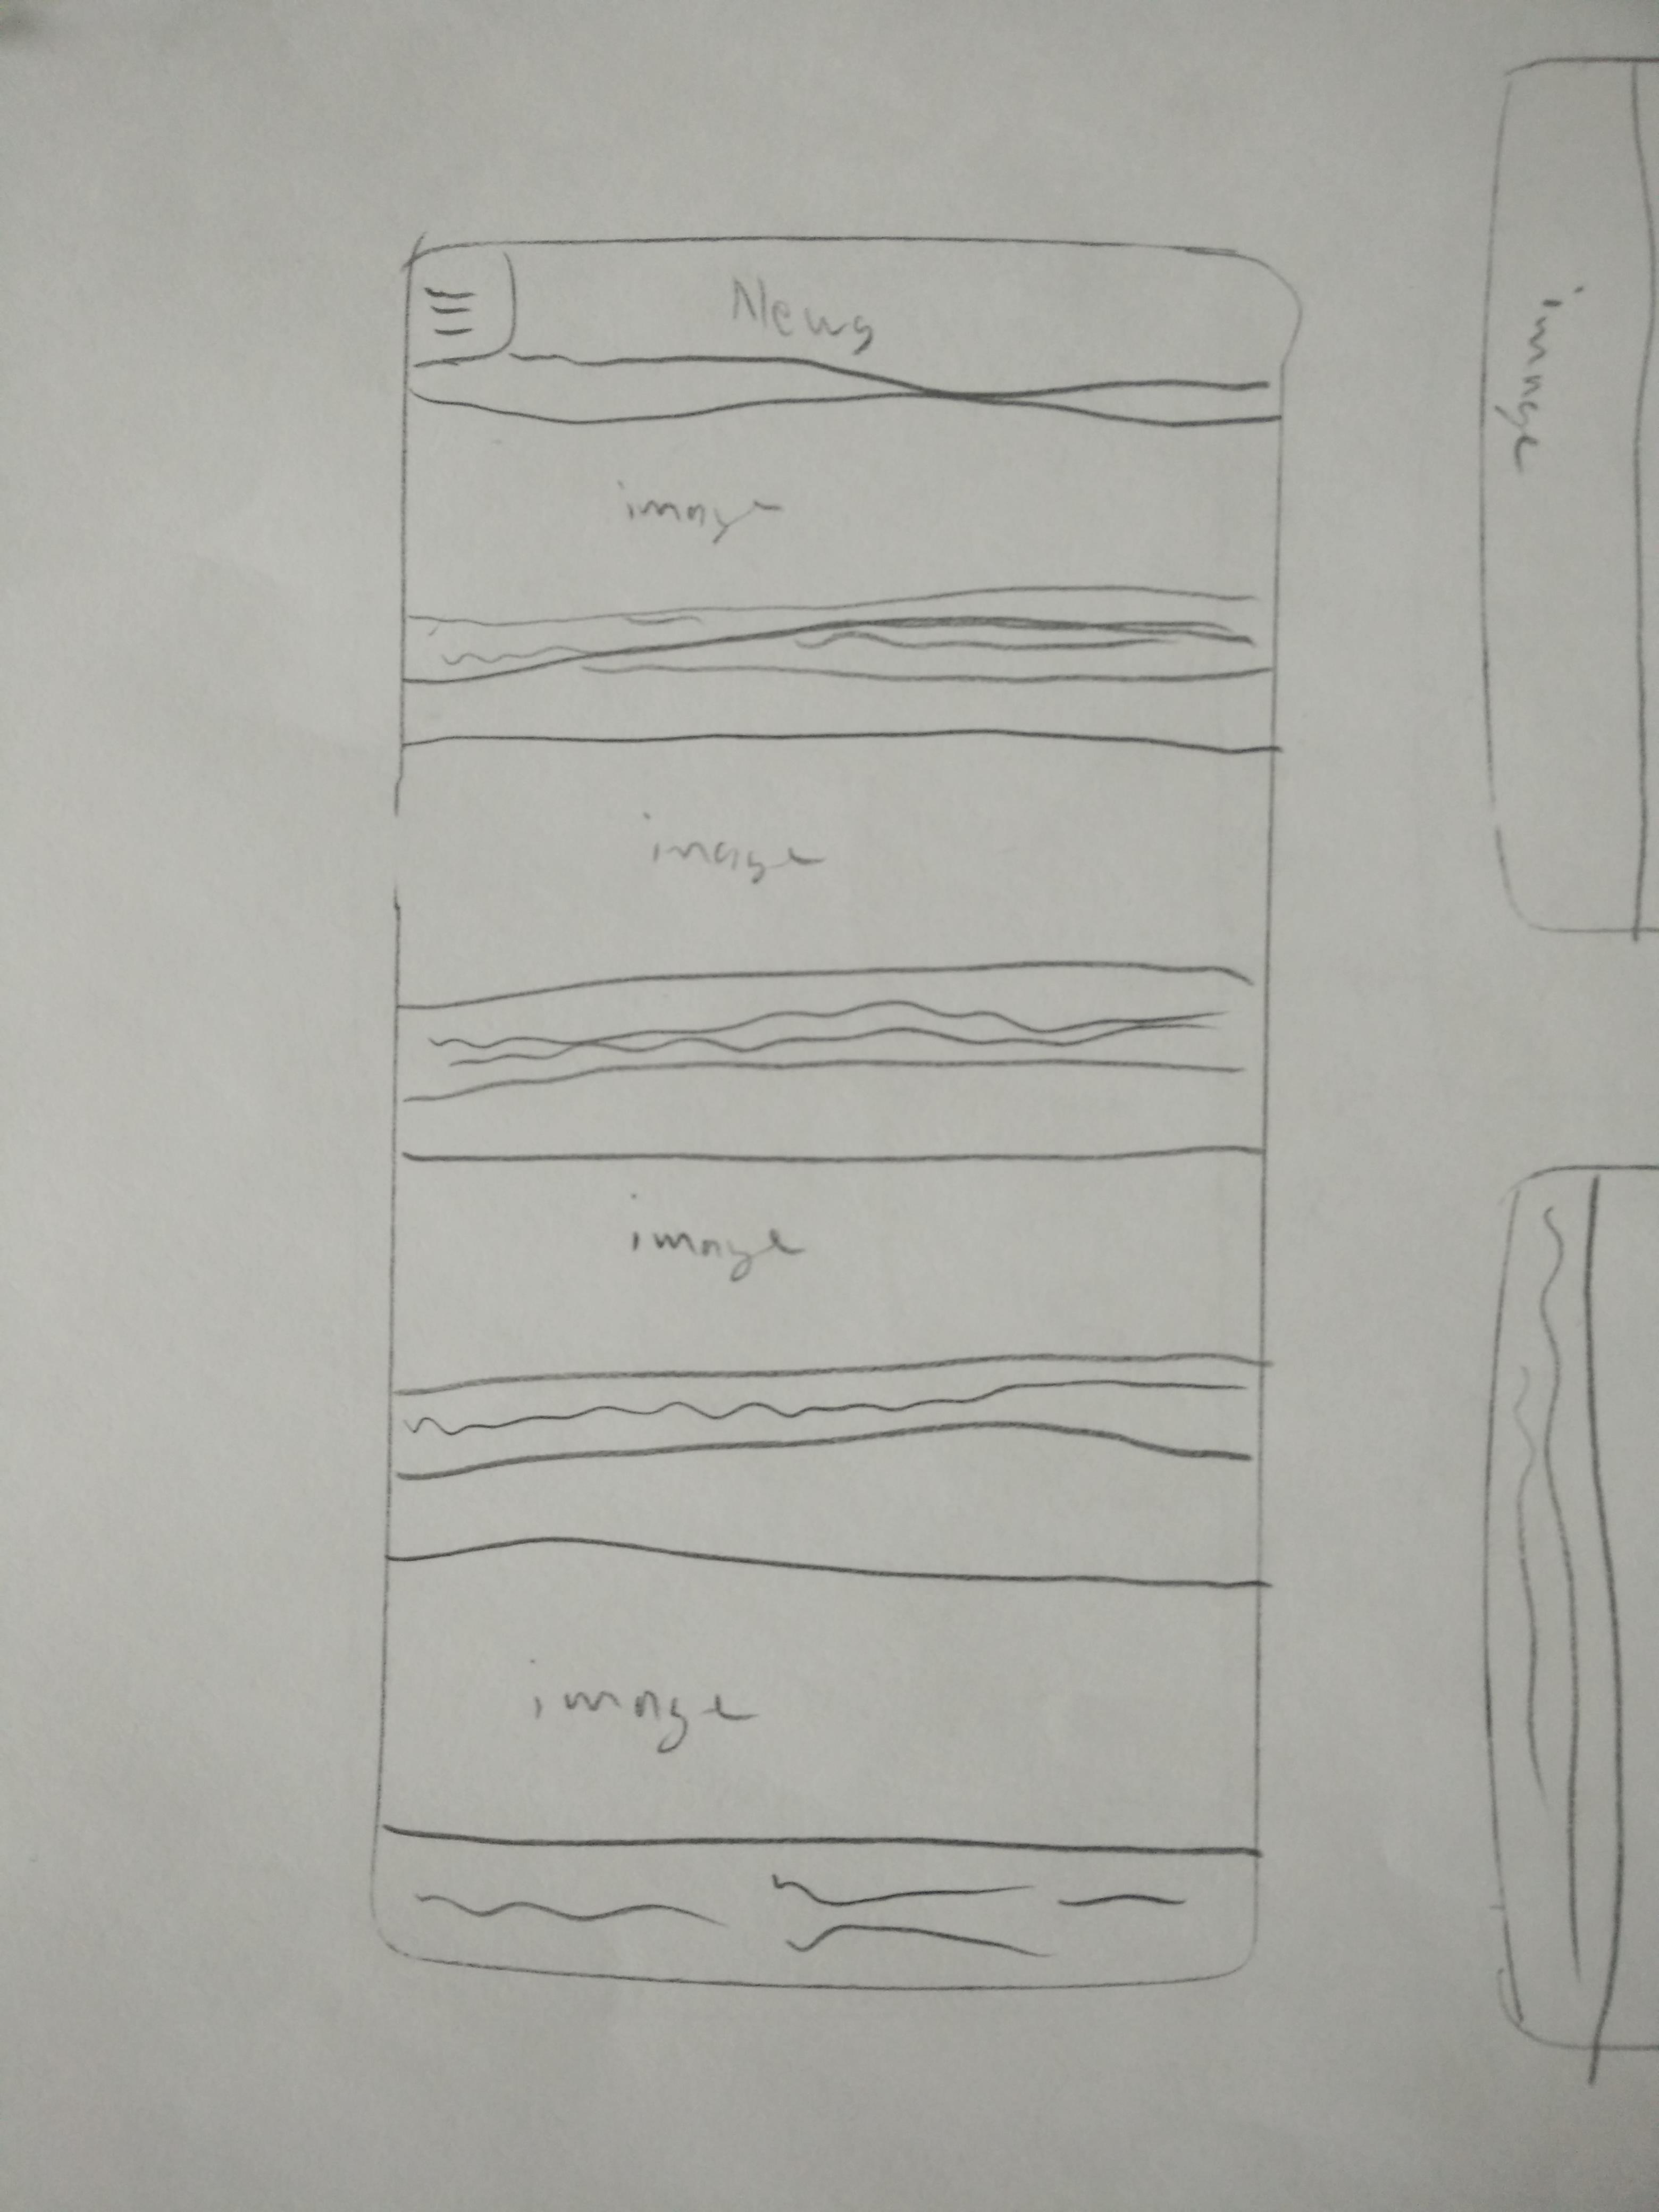
\includegraphics[height=\textheight/2]{sketches 02}
  \caption{Sketch 2}
  \label{fig:sketch-02}
\end{figure}

Dieser Sketch wurde ausgewählt, weil er enorm Sektminimalistisch ist, sodass der kleine Screen eines mobilen Gerätes maximal viel Inhalt bieten kann, da kein Platz für Navigationsleisten in Anspruch genommen wird. Damit einher geht auch ein hoher Grad an Übersichtlichkeit. Problematisch ist aber einerseits, dass trotz nicht vorhandener Menüleiste aufgrund der großen Bilder recht wenig Text untergebracht werden und andererseits, dass zu sämtlichen anderen Screens beziehungsweise Funktionalitäten nur umständlich über das \enquote{Burgermenü} navigiert werden kann. Dies ist wenig intuitiv und könnte den User sehr schnell von unserem Produkt abringen, da er nicht auf den ersten Blick findet, was er sucht und er den Funktionsumfang der App schwer einschätzen kann. Gerade beim erstmaligen öffnen der App würde dies möglicherweise viele Interessenten dazu bringen, die App sofort wieder zu deinstallieren, zumal der Sketch designmäßig recht pragmatisch und wenig ausgefeilt wirkt. Die Stärke dieses Sketches ist also gleichzeitig auch seine größte Schwäche. Er erinnert uns aber daran, platzsparend mit Navigationselementen umzugehen.

\subsection{Sketch 3}

\begin{figure}[h]
  \centering
  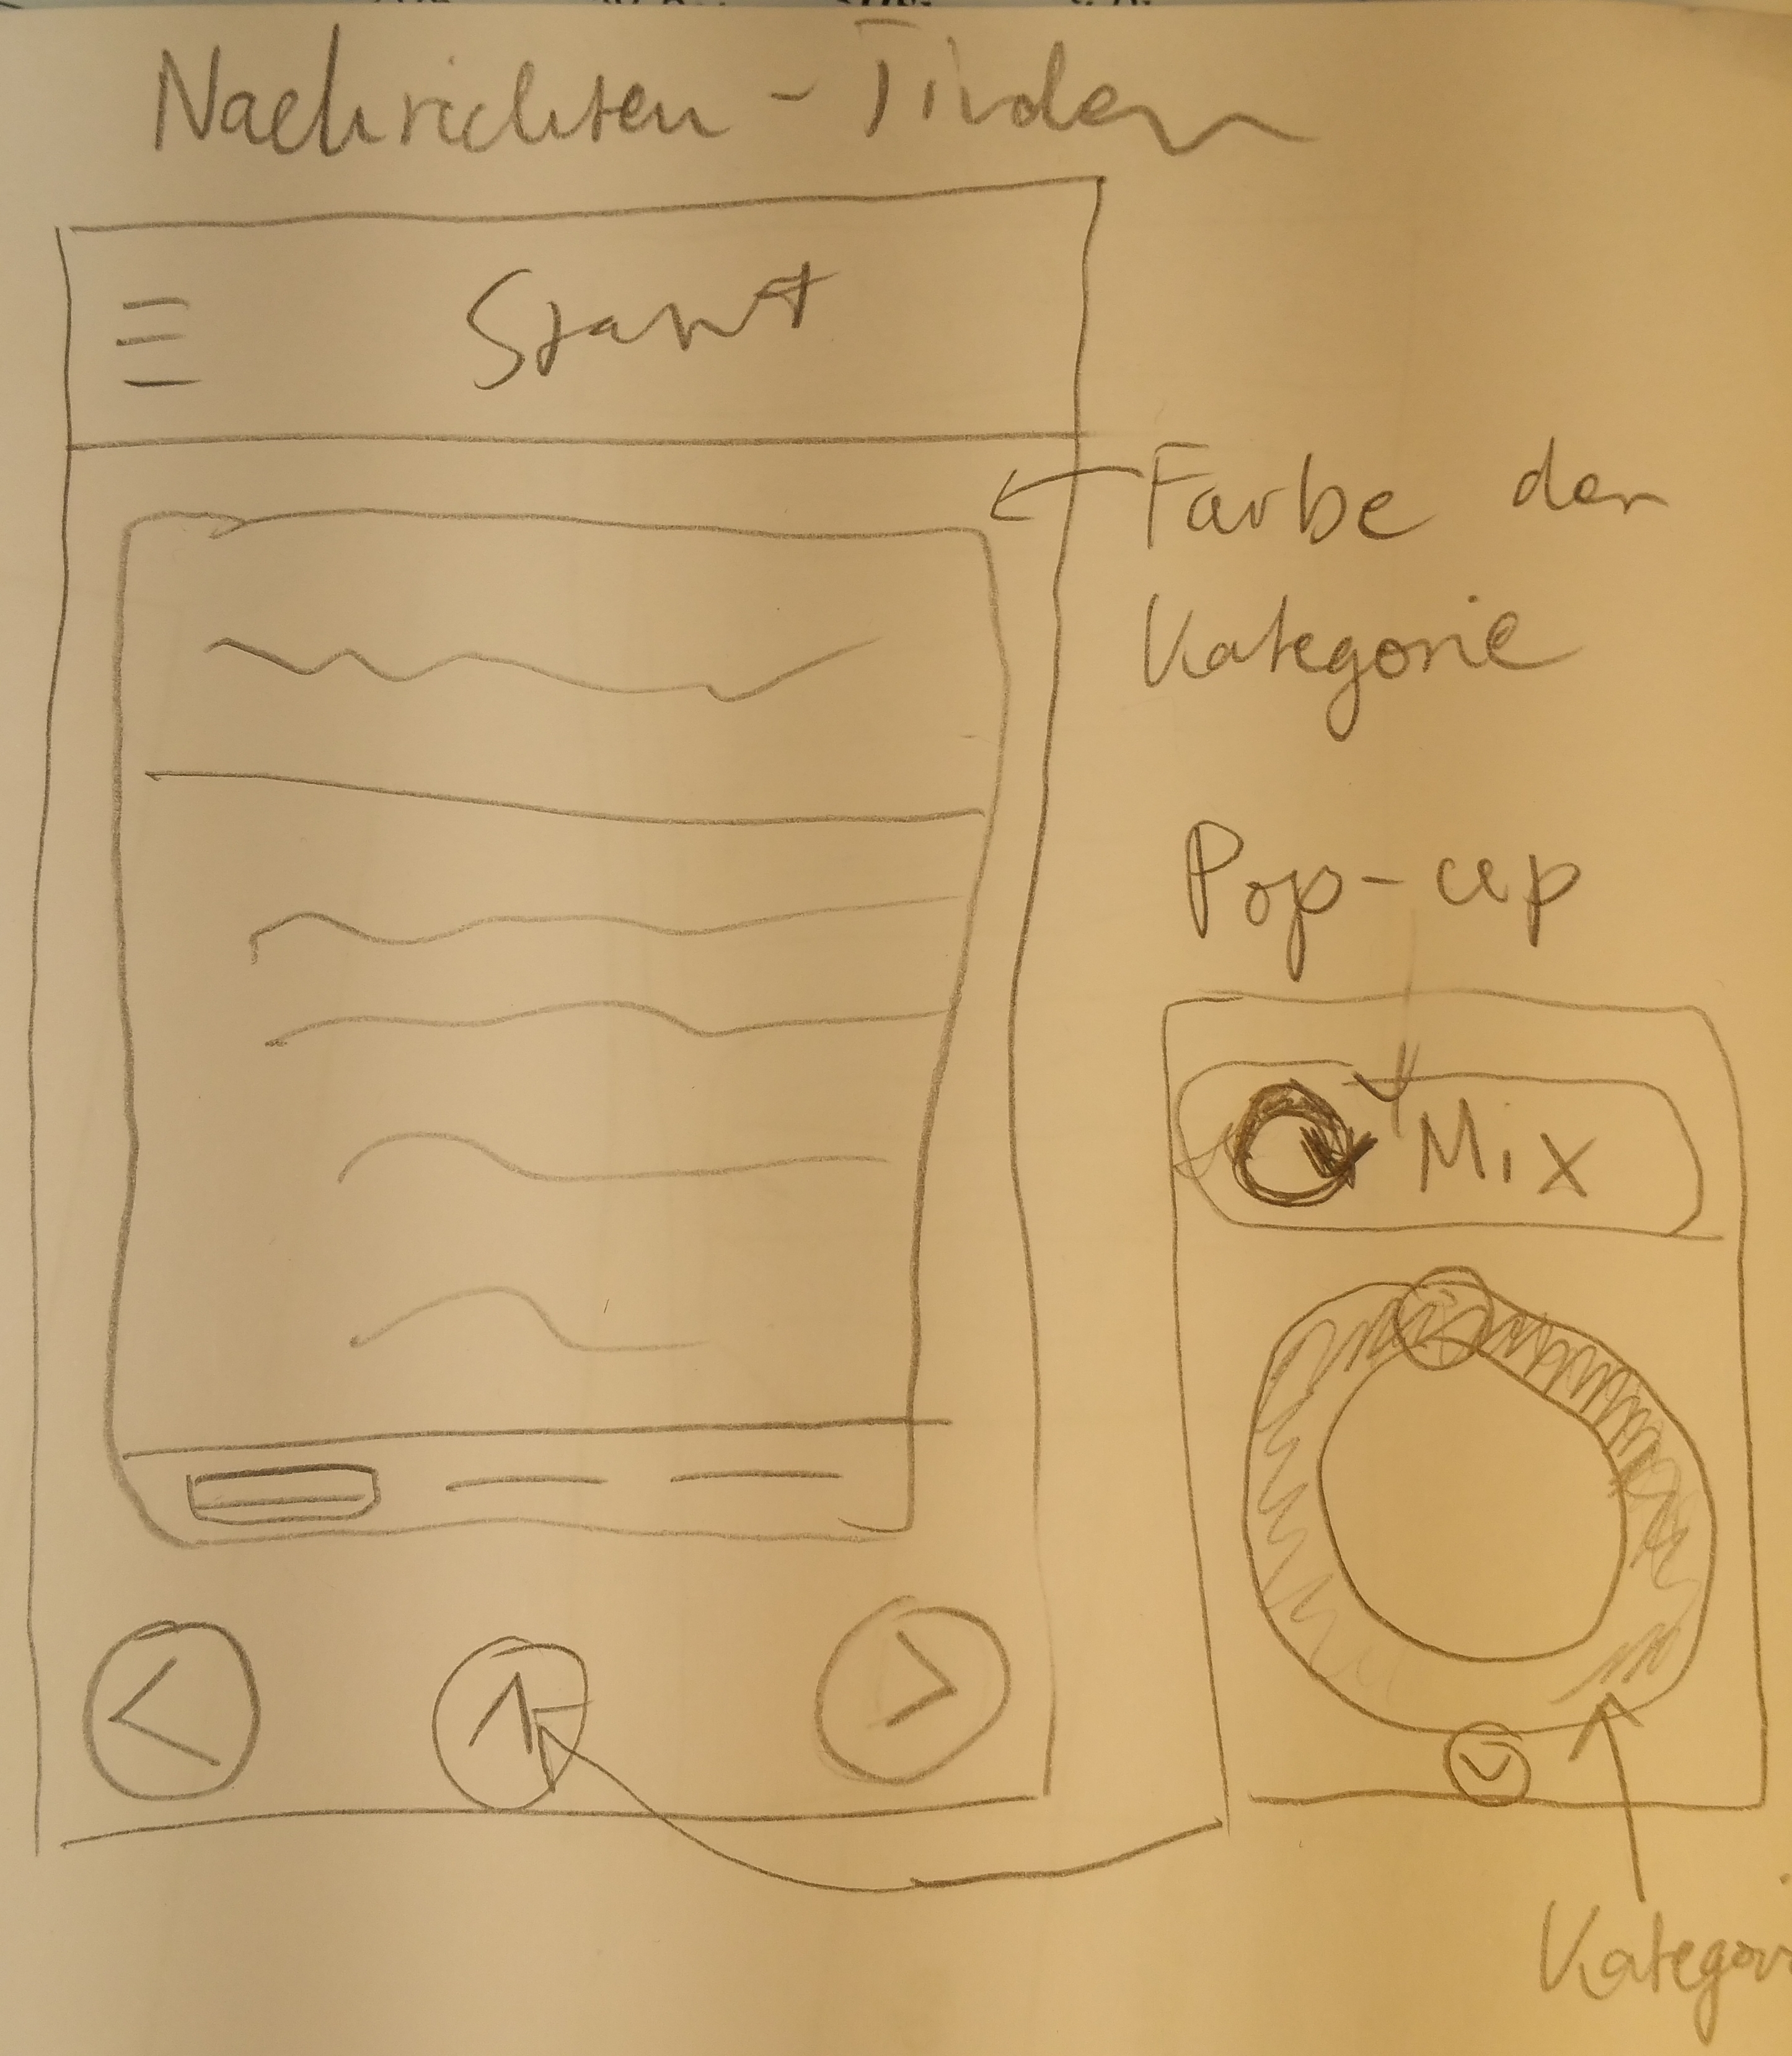
\includegraphics[height=\textheight/2]{sketches 03}
  \caption{Sketch 3}
  \label{fig:sketch-03}
\end{figure}

Dieser Sketch bringt ein abweichendes, aber sehr interessantes Bedienkonzept ein, nämlich eines, das sich stark an der berühmten \enquote{Tinder}-App orientiert. Dieses möchten wir auf jeden Fall in die Explore-Funktion unserer App integrieren, da dies ein Feature darstellt, welches bisher keine andere App dieses Genres bietet und vor allem das jüngere Publikum ansprechen dürfte. Aber auch für ältere Personen ist es ein leicht zu verstehendes, innovatives Konzept.

\subsection{Sketch 4}

\begin{figure}[H]
  \centering
  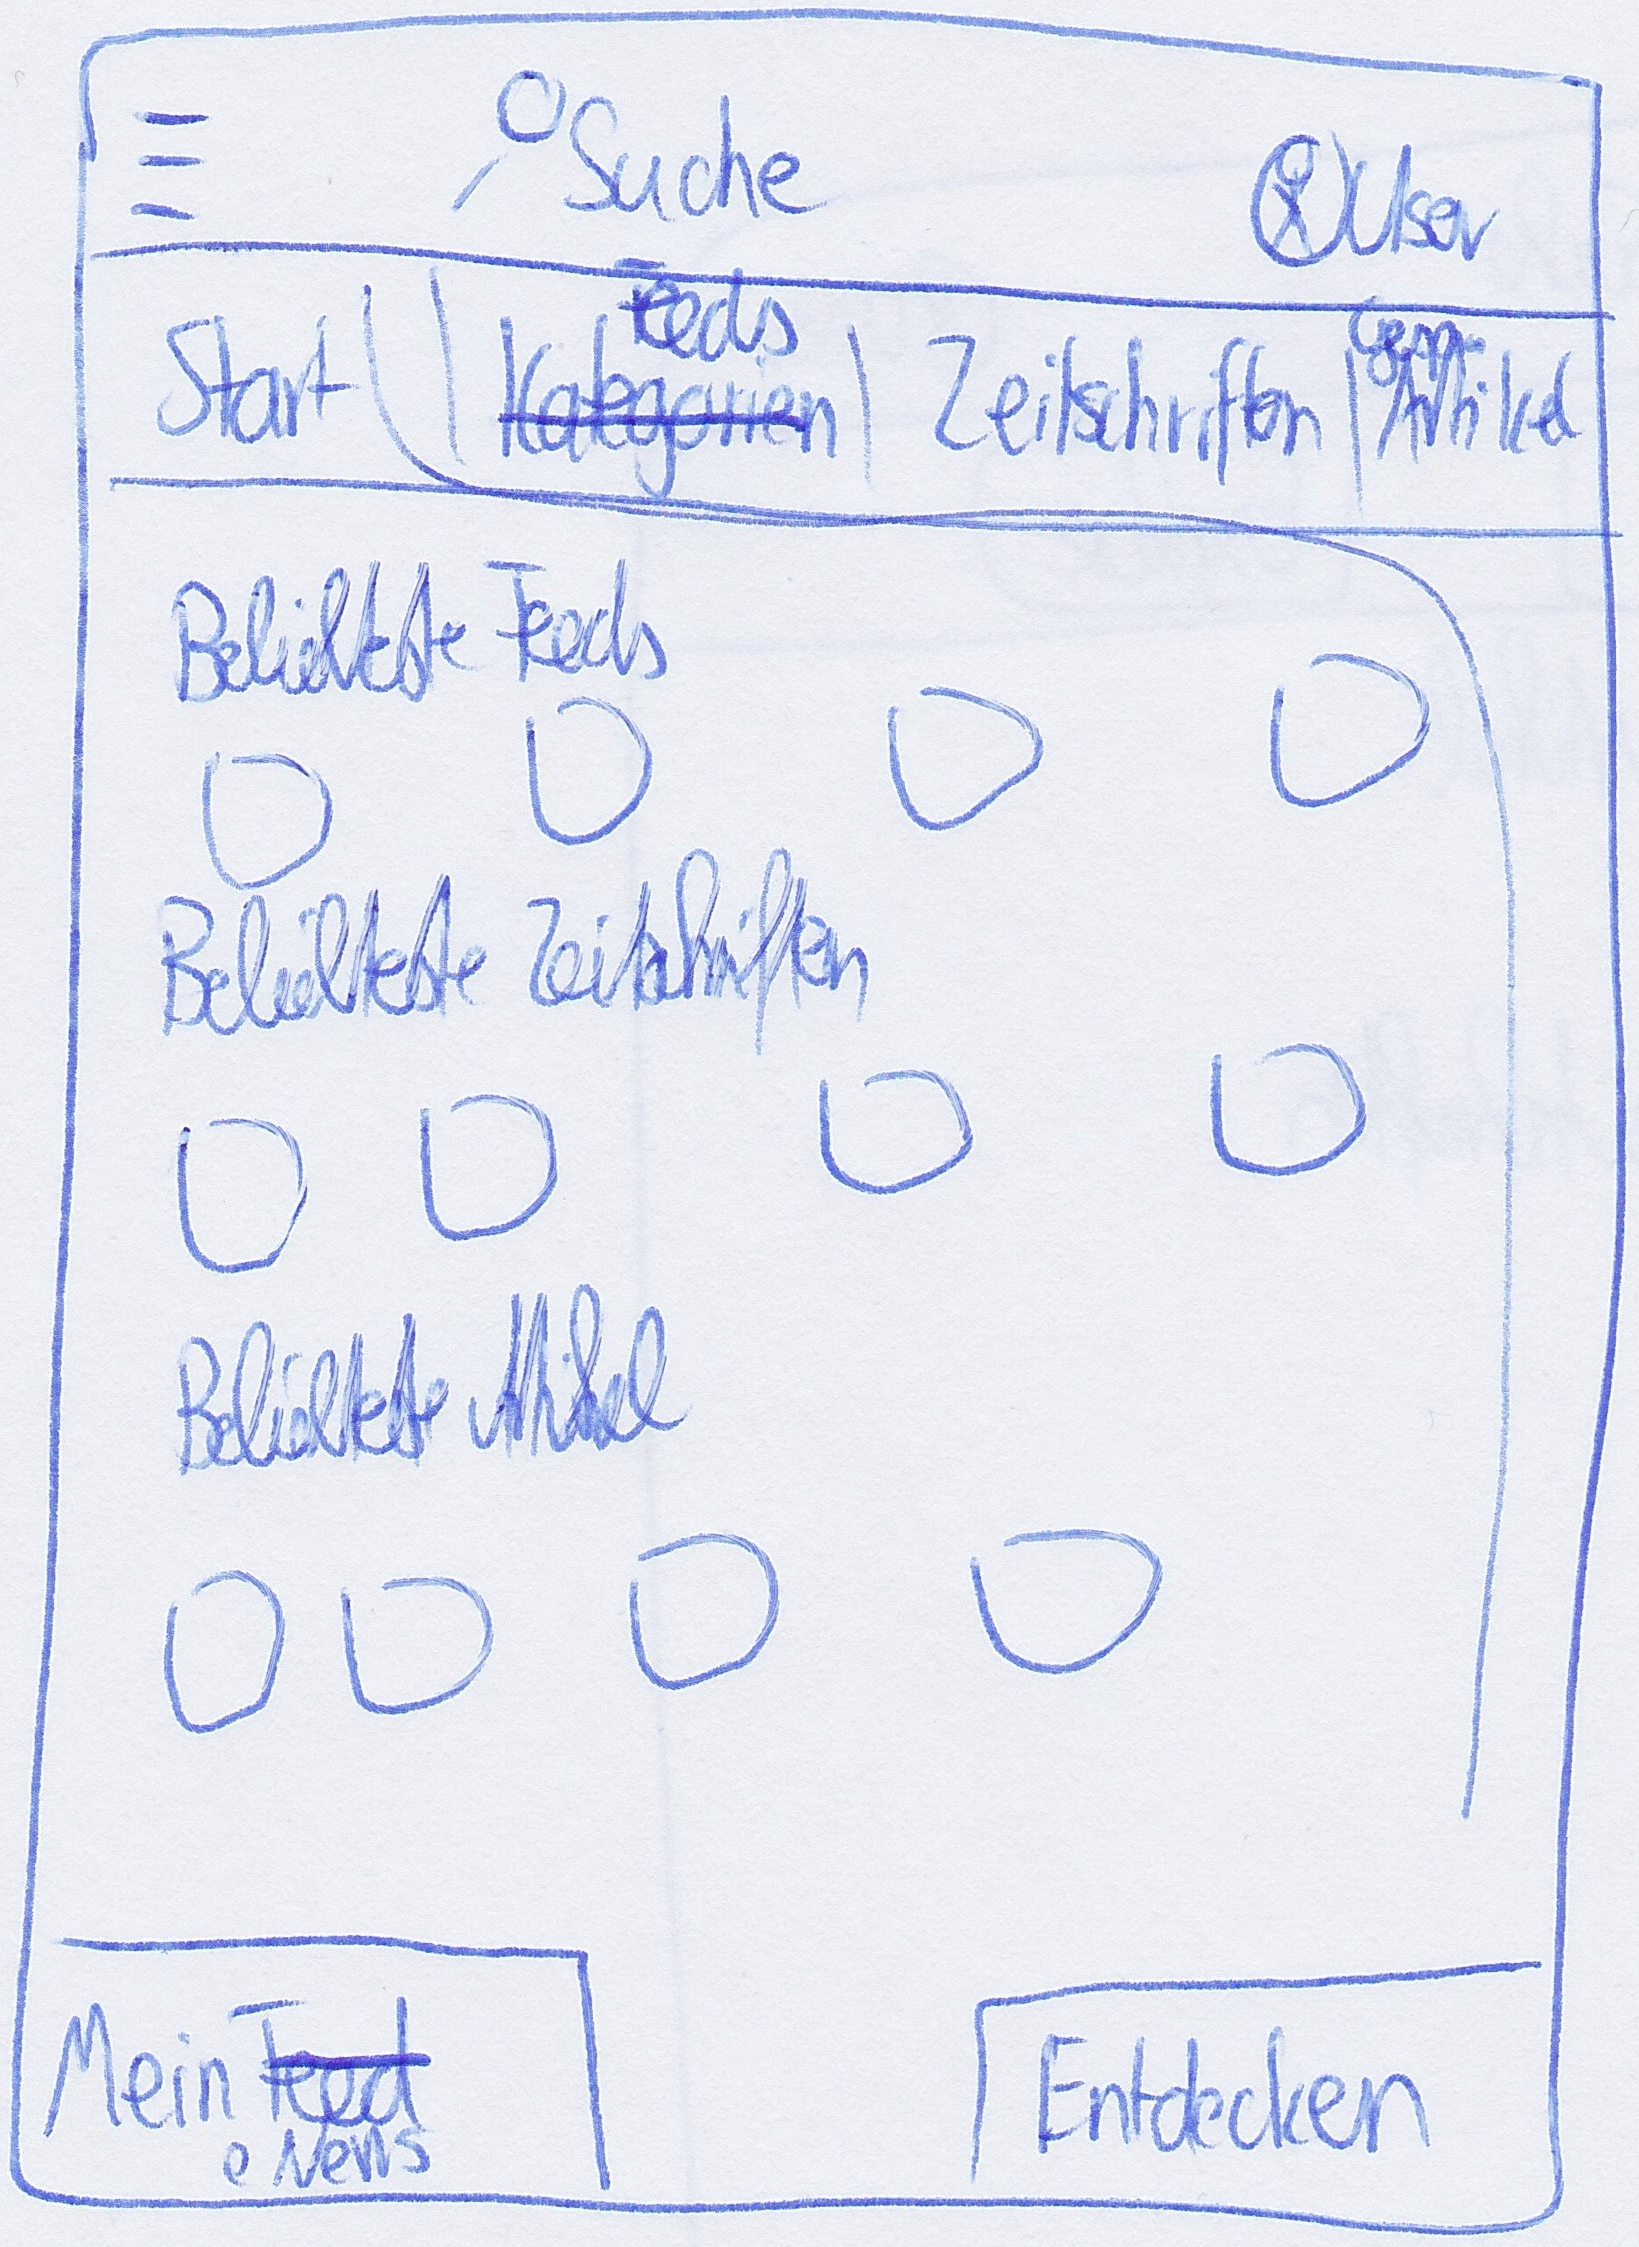
\includegraphics[height=\textheight/2]{sketches 04}
  \caption{Sketch 4}
  \label{fig:sketch-04}
\end{figure}

Dieser Sketch bringt einen hohen Grad an Funktionalität, sowie eine Navigationsmöglichkeit über Tabs ein. Problematisch an ihm sind die vielen Navigationselemente (Navigationsleiste unten, Tabs, Profil, Suche, Burgermenü), sodass möglicherweise die Übersichtlichkeit verloren geht und der User zunächst überfordert ist. Die Idee der einzelnen Tabs möchten wir aber auf jeden Fall in unseren Prototypen übernehmen, da sie mehrere Vorteile gegenüber anderen Navigationskonzepten besitzen. Unter anderem ist diese Form der Navigation schon aus vielen anderen Apps bekannt, sodass der User sich von Beginn an recht heimisch fühlen dürfte. Weiterhin suggerieren Tabs schon beim ersten Aufruf der App die Kernfunktionalitäten und geben ihr somit auf verständliche Weise Struktur. Zuletzt ist die Navigation mit ihnen auch sehr zügig möglich.

    % !TeX encoding=utf8
% !TeX spellcheck=de-DE
% !TeX root=../UID_Project_Documentation.tex

\section{Prototyping}

\subsection{Entwicklung des Prototypen}

Aus den verschiedenen Ideen die durch die Sketches aufgezeigt wurden, wurde dann der Prototyp entwickelt. Uns war wichtig das der Gulf of Execution und Gulf of Evaluation konsistent sind und die Benutzer der Anwendung durch unvorhersehbares Verhalten verwirren oder sogar frustrieren. Wir haben uns bei dem Prototyp für eine Android App entschieden, da aufgrund der Marktanalyse Smartphone Apps für Online Nachrichten den größten Marktanteil haben. Android aus dem Grund, da Android für uns eine bekannte Umgebung ist und mittlerweile den größten Marktanteil hat. Diese Entscheidung könnte aber auch zu Nachteilen bei den User Tests führen, falls die Testpersonen des User Test iPhone Benutzer sind.

Die App hat einen Hauptbereich in dem die Haupt Funktionalität angesiedelt ist. In diesem Bereich geht es nur um die Nachrichten, das Erkunden und die \enquote{Feeds}, welche den Kern der App darstellen. Die Navigation funktioniert über eine Tab-Leiste, welche immer sichtbar ist.

Bewusst Abgetrennt sind die persönlichen Daten des Benutzers, die sich über das \enquote{Burger}-Menü öffnen lassen. Von diesem Menü kann der Benutzer zu verschiedenen Übersichten Navigieren, die beispielsweise die abgeschlossenen Abonnements anzeigen. Durch diese Anordnung wollten wir verdeutlichen, das es sich eher um sekundäre Funktionen handelt, die nichts mit den eigentlichen Nachrichten zu tun hat. Diese Gestaltung basiert auf Sketch 3 in Abbildung \ref{fig:sketch-03}.

Die Home Ansicht zeigt einen Default-Feed an, der aus den eigenen Feeds ausgewählt werden kann. Hier werden die Nachrichten jeweils mit Bild und der Schlagzeile angezeigt. Die Nachrichten sollen in einer möglich kurzen Form präsentiert werden. Es wäre auch möglich dies ohne das Bild zu einer Nachricht zu machen, aber da Menschen primär den Sehsinn verwenden, war unseres Erachtens nach die Variante mit Bild und Schlagzeile angenehmer als nur Text. Die Gestaltung dieser Ansicht basiert auf Sketch 2 in Abbildung \ref{fig:sketch-02}.

In der Customize Ansicht werden alle Feeds aufgelistet und es gibt die Möglichkeit einen neuen Feed anzulegen. Das Anlegen der Feeds wird über einen sogenannten \enquote{Floating-Action-Button} angestoßen. Wir haben uns dafür entschieden dies so zu realisieren, da es unserer Ansicht nach deutlich signalisiert, das dieser Button dort ist, um etwas neues anzulegen. Viele Android Apps, unter anderem WhatsApp, gehen einen ähnlichen Weg, wenn es darum geht neue Inhalte anzulegen. Die tatsächliche Ansicht zur Anpassung der Feeds wird mit einem Klick auf das jeweilige Listen Item geöffnet. Die Grundidee für dieses Ansicht lieferte Sketch 4 in Abbildung \ref{fig:sketch-04}. Es wurde in abgewandelter Form die Auflistung übernommen.

Bei dem Konfigurieren oder Erstellen eines neuen Inhalts wird eine Übersicht der vorhandenen digitalen Nachrichtenangebote angezeigt. Ein Checkbox bei jedem Nachrichtenangebot signalisiert, ob diese Quelle für den aktuellen Feed ausgewählt wurde. Ein Schloss-Piktogramm bei dem Item neben der Checkbox signalisiert, dass es sich um einen nicht erworbenen, kostenpflichtigen Anbieter handelt. Wir haben uns an der Stelle für ein Piktogramm anstatt Text entschieden, da wir denken, dass Benutzer so schneller den Sachverhalt wahrnehmen und auch die Gestaltung übersichtlicher ist. Durch einen Klick auf den Nachrichtenanbieter wird eine Übersicht der Kategorien angezeigt, die ein Nachrichtenanbieter anbietet. Ebenso wie der Anbieter übersicht ist eine Checkbox der Indikator zur Auswahl und ein Schloss-Piktogramm signalisiert kostenpflichtige Inhalte. Wenn ein Benutzer kostenpflichtige Inhalte hinzufügt, muss er noch den Kauf bestätigen. Dies geschieht durch ein Popup, welches dem Benutzer zeigen soll, was er/sie mit seiner Handlung verursacht und welche Konsequenzen es hat. Dies geschieht in dem Hinblick Gulf of Execution und Gulf of Evaluation zusammenzubringen. Wir haben uns für diese zweistufige Auswahl der Inhalte entschieden, da es unser Erachtens so den Benutzern eine gute, nicht überladene Übersicht gibt. Mehr Funktionalität, oder ausklappbare Inhalte könnten unerfahrene Benutzer verwirren. Am unteren Rand der View ist ein Button zum speichern, welcher farblich gegenüber den Listen Items abgehoben ist. Seine Funktionalität ist das Speichern. Es soll durch die andere Farbe verdeutlicht werden, dass der Benutzer durch Interaktion mit dem Button die Ansicht verlässt und zur vorherigen Ansicht zurückkehrt und die Daten gespeichert werden.

Die Explore Ansicht dient zur Erkundung von neuen Inhalten und soll bei den Benutzern das Interesse wecken kostenpflichtige Inhalte zu abonnieren. Die Grundidee kommt aus Sketch 3 in Abbildung \ref{fig:sketch-03}. Außerdem orientiert sich die Gestaltung an der Tinder App. Wir haben das Konzept von Tinder abgewandelt, da Nachrichten unseres erachtens nach eine etwas andere Darstellung brauchen als Personen in einer Dating App. Es gibt einen Button zum Anzeigen des aktuellen Artikels und einen Button zum anzeigen des nächsten Artikels. Die Button unterscheiden sich farblich von einander, um die Funktionalität visuell abzugrenzen. In dieser Übersicht werden von der Nachricht grundlegende Informationen angezeigt: Bild, Schlagzeile, Zeitung/Quelle, Resort. Ähnlich wie bei der Home Ansicht war der Gedanke hierbei die Nachricht zu kurz wie möglich zu präsentieren. Die Gestaltung einer Vollbild Ansicht einer einzigen Nachricht wurde gewählt, da es bei der Explore Ansicht explizit um das erkunden einzelner neuer Inhalte für den Benutzer geht. Der Benutzer soll sich dadurch auch die Zeit nehmen und von nichts anderem abgelenkt werden, wenn sich ein Nutzer neue Inhalte anschaut. Wenn der Benutzer sich dazu entscheidet einen Artikel zu lesen, kann er am Ende des Artikels die Quelle mit der Kategorie zu einem seiner Feeds mit einem Button hinzufügen.

Generell haben wir also sehr viel Wert darauf gelegt, die App übersichtlich und leicht benutzbar zu gestalten, sodass auch Personen, die weniger souverän im Umgang mit Smartphones sind, also unserer Persona \enquote{Uli} ähnlich sind, nicht überfordert oder sogar frustriert werden. Dabei wollten wir aber nicht schnellere User (also technikaffine Personen, die der Persona \enquote{Sabine} ähneln) durch unnötig viele Unterbrechungen in Form von Popups oder ähnlichem ausbremsen, sondern diese nur dort einbauen, wo es sinnvoll ist, nämlich wenn zahlungspflichtige Käufe getätigt werden. Dieser Art von Benutzern sollte die Bedienung der App zudem ohnehin leicht fallen, da wir uns an den typischen Android-Design-Paradigmen orientiert haben.

\subsection{Flow Chart}

\begin{figure}[H]
  \centering
  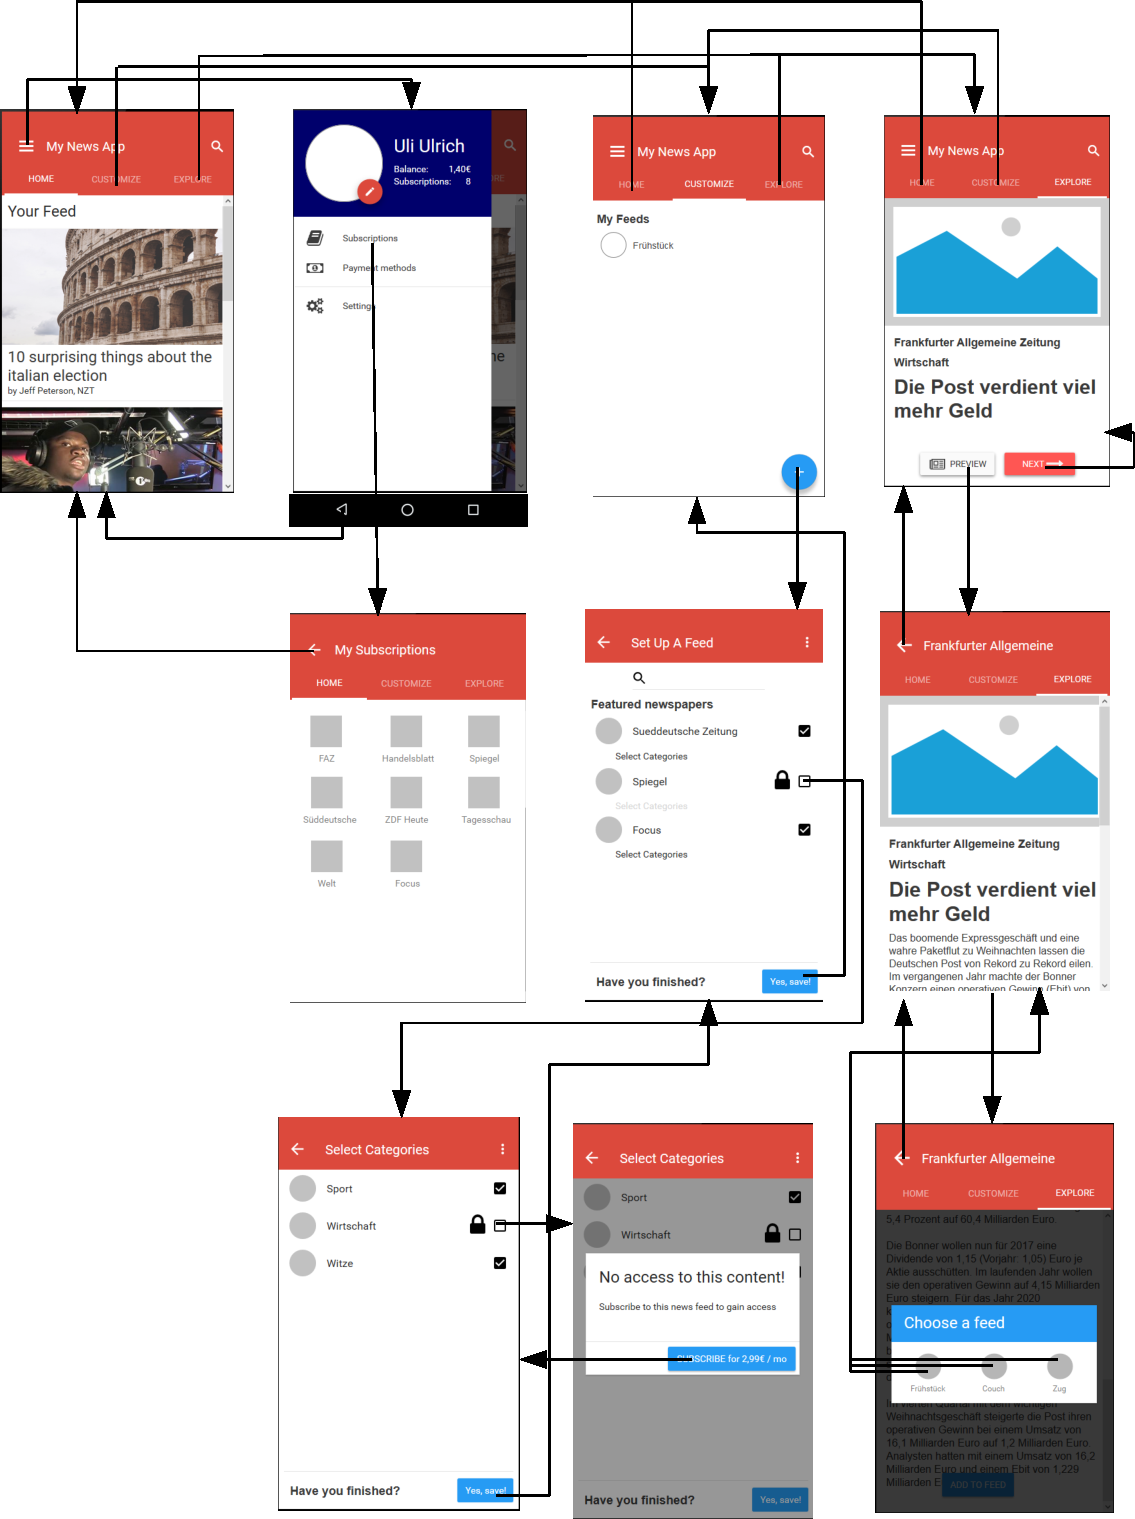
\includegraphics[width=\textwidth]{flowchart}
  \caption{Flowchart der MyNewsApp}
  \label{fig:flowchart}
\end{figure}

    % !TeX encoding=utf8
% !TeX spellcheck=de-DE
% !TeX root=../UID_Project_Documentation.tex

\section{Evaluation: User Tests}

\subsection{Ziele}

Ziel unseres User Tests war in erster Linie festzustellen, ob unser USP, also ein granulares, vollständig individuell zusammenstellbares Nachrichtenangebot, instantan erkannt wird.

Zudem wollten wir feststellen, ob das Prinzip der Feeds grundsätzlich verstanden wird und deren Umsetzung intuitiv für den Nutzer ist. Dies war uns sehr wichtig, da nur mit Feeds das Potenzial der App zum Tragen kommt. Ist deren Sinn unklar oder die Erstellung zu kompliziert, erlischt einer unserer größten Vorteile im Vergleich zu Konkurrenzprodukten.

Ein sehr generelles Ziel war aber natürlich auch Probleme bei der Nutzung herauszufinden und somit Schwachstellen in der Bedienbarkeit zu beseitigen.

\subsection{Testprobanden}

Unsere Testprobanden setzten sich zusammen aus fünf Studenten im Alter von etwa 20 Jahren, die unterschiedliche Erfahrungsstände in Bezug auf Nachrichtenapps haben.

Proband 1 ist weiblich, absolviert ein Studium mit Schwerpunkt Medien und pendelt, zur Zeit aber mit dem Auto, jedes Wochenende 70 km. Es ist aber denkbar, dass sie in naher Zukunft den Zug nutzen wird, sodass sie dort dann eventuell Nachrichten konsumieren möchte. Proband 1 hat bisher allerdings keine Erfahrung mit News-Apps.

Proband 2 und 3 sind ebenfalls weiblich und studieren dual an der DHBW Karlsruhe. Sie haben einen starken Bezug zu Technik und Smartphones. Auch Proband 5, allerdings männlich, interessiert sich sehr stark für neue Technologien und Entwicklungen, da er ein Studium im Bereich Informatik absolviert.

Proband 4 studiert Architektur, hat aber im Vergleich zu allen anderen Probanden keine große Affinität zu Technik, weshalb dieser Kandidat besonders wichtig für unseren User Test war.

Lediglich Proband 3 nutzt bisher eine App, um sich über aktuelle Geschehnisse und Nachrichten zu informieren.

Die meisten unserer Probanden entsprechen stark der Persona von Sabine, da sie einerseits technikaffin sind, andererseits aber auch ein begrenztes Einkommen haben. Zudem sind sie sehr gebildet und aufgrund ihres Studiums ist Zeit wohl das am meisten knappe Gut.

Leider konnten wir keine Person mittleren Alters zu einem User Test bewegen. Wir sind aber der Meinung, dass wir eine ausreichend unerfahrene und technik-averse Person einbringen konnten (Proband 4), die uns ähnliche Resultate wie eine an der Persona \enquote{Uli} ausgerichtete Person liefern dürfte.

\subsection{Gestellte Fragen und Aufgaben}

Um festzustellen, ob unsere Navigationselemente in Form von Tabs aussagekräftig genug sind und dem User von Anfang an klar machen, was die Besonderheit unserer App ist, fragten wir noch vor allen anderen Aufgaben und Fragen, welche Funktionalitäten bei Betrachten der Action Bar erwartet von ihnen erwartet werden.

Die erste Aufgabe bestand dann darin, einen Feed zu erstellen. Diese Aufgabe zielte einerseits darauf ab, zu erkennen, ob Feeds generell verstanden werden, andererseits aber auch darauf, ob ihre Erstellung einleuchtend ist.

Weitere Aufgaben und Fragen sollten dann aufzeigen, ob es sonstige Probleme mit der Bedienung , sowie Navigation gibt und uns noch einmal zeigen, ob der USP tatsächlich vollständig verstanden wurde.

Der vollständige Moderationsleitfaden mit allen Aufgaben und Fragen, sowie der Moderation an sich, ist im Anhang dieser Projektdokumentation zu finden.

\subsection{Ergebnis}

Der User Test hat gezeigt, dass unser USP im großen und Ganzen von den Usern enorm schnell erkannt wird. Ohne sich mit der App befasst zu haben, wurde von den meisten Testprobanden anhand der Tabs erkannt, dass das Nachrichtenangebot individualisierbar ist. Dies war im positiven Sinne überraschend.

Es wurde zudem recht schnell klar, dass Android Nutzer mit dem Design sehr schnell vertraut sind und instinktiv zu den geforderten beziehungsweise gewünschten Screens navigieren.

Vereinzelt gab es aber Probleme mit der Auswahl der Kategorien einzelner Zeitungen beim Erstellen bzw. Bearbeiten eines Feeds. Die Auswahlmöglichkeit wurde hier oftmals entweder übersehen oder nicht verstanden.

Beim Abonnieren von Inhalten im Explore-Modus wurde zudem erwartet, dass der dafür zuständige Button nicht am Artikelende, sondern im Kopfbereich des Screens positioniert ist.

Es wurde außerdem klar, dass die Feeds, welche standardmäßig erstellt sind, darunter zum Beispiel \enquote{Frühstück}, dazu führen, dass der User möglicherweise den Sinn der Feeds nicht begreift. Argumentiert wurde zum Beispiel, dass man morgens keine anderen Interessen hat, als beispielsweise abends, sodass ein Feed explizit für den Morgen sinnfrei ist.

Da die Zurück-navigieren-Funktion beim ersten Prototypen noch nicht vollständig implementiert war, entstand auch hierbei Verwirrung.

\subsection{Abgeleitete Verbesserungsmaßnahmen}

Aus den entstandenen Problemen und Schwierigkeiten wurden die folgenden Verbesserungsvorschläge abgeleitet.

Zunächst möchten wir natürlich die Problematik betreffend die Auswahl der Kategorien beim Erstellen von Feeds lösen. Dies geschieht durch eine verbesserte Menüführung, die nach einem neuen Prinzip funktioniert. Als ersten Auswahlschritt sieht der Benutzer alle Nachrichtenquellen und hat die Möglichkeit nach diesen zu suchen oder auch nach Kategorien zu filtern. Im zweiten Schritt kann der Benutzer dann Kategorien hinzufügen. Hat der Benutzer eine Kategorie aus einer Nachrichtenquelle selektiert, so sieht er einen Haken neben dem entsprechenden Titel auf der Übersichtsseite, um direkt zu erkennen, dass eine Kategorie in diesem Untermenü ausgewählt wurde. Um den neuen Feed zu speichern, wird ein Disketten-Symbol an dem für Android typischen Platz eingeführt.

Weiterhin werden wir die standardmäßig, vordefinierten Feeds durch aussagekräftigere, sowie sinnhaftere ersetzen.

Den Button, der dafür zuständig ist, Inhalte aus dem Explore-Modus heraus zu abonnieren, soll nun auch im Kopfbereich eines Artikels angezeigt werden, sodass er leichter gefunden werden kann. Dies sollte analog zu den Änderungen in anderen Ansichten durch ein neues Piktogramm in der Menüleiste umgesetzt werden.

Natürlich werden wir auch die Navigation, insbesondere das Zurück-navigieren verbessern, respektive vollständig implementieren.
Zudem wurden uns noch einige interessante Impulse bezüglich Funktionen der App gegeben. So sollte es eine Möglichkeit geben, nach Ländern oder Regionen zu filtern, sowie den Homescreen zu personalisieren, in dem man entscheidet, welche Artikel angezeigt werden.

Umsetzen möchten wir aber noch die Filtermöglichkeit nach Regionen beziehungsweise Ländern, da dies eine von uns bisher versäumte, aber sehr grundlegende Funktionalität darstellt.

Mit diesem Schritt im UCD-Prozess ist nun ein gesamter Zyklus durchlaufen worden, sodass im folgenden Kapitel die erste Iteration erfolgen kann.

    % !TeX encoding=utf8
% !TeX spellcheck=de-DE
% !TeX root=../UID_Project_Documentation.tex

\section{Iteration}

Die bereits im Kapitel \enquote{User Test} diskutierten Verbesserungsmaßnahmen wurden erwartungsgemäß umgesetzt.
Zusätzlich haben wir aber noch von uns aus einige Anpassungen vorgenommen, welche auch in Bezug auf die Vorlesungseinheit \enquote{Mobile UX} aufkamen.

Da der Nutzer auf einem mobilen Gerät aller Wahrscheinlichkeit nach mehrere Apps nebenbei geöffnet hat und er somit auch sehr stark abgelenkt ist, ist es wichtig, dass er zu jedem Zeitpunkt, an dem er wieder zu unserer App zurückwechselt, genau weiß, wo er sich befindet. Um dieses \enquote{Design for interrupts}-Paradigma zu berücksichtigen, haben wir uns dazu entschlossen, in der Action Bar jedem Screen einen entsprechenden Titel zu geben. Wenn man also beispielsweise einen Feed erstellt, und eine Zeitung ausgewählt hat, sodass man nun die Kategorien auswählen muss, steht in der Action Bar der Titel der Zeitung, für welche man die Kategorien auswählt.

\begin{wrapfigure}{R}{0.45\textwidth}
  \centering
  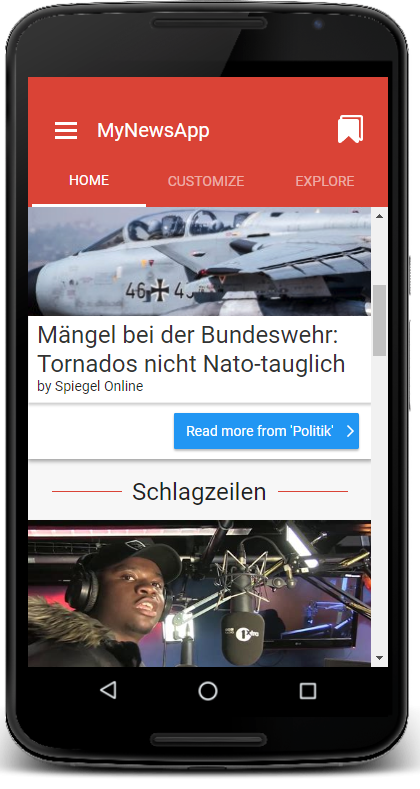
\includegraphics[width=0.4\textwidth]{screenshot 01}
  \caption{\enquote{Home} Ansicht der MyNewsApp}
  \label{fig:screenshot-01}
\end{wrapfigure}

Um mehr Übersichtlichkeit auf dem Homescreen zu schaffen, haben wir eine besser erkennbare Untertrennung der einzelnen Feeds umgesetzt. Feedüberschriften sind vom Rest des Textes abgesetzt und durch minimale Farbwechsel des Hintergrunds bei jedem Feed kann man auch bei schnellem Scrollen schnell erkennen wo die Feeds beginnen und aufhören. Die Buttons, die dafür zuständig sind, mehr von einem Feed anzuzeigen, sind ebenso auffälliger.

Um die gespeicherten Inhalte schneller zu erreichen, wurde der \enquote{Saved Articles}-Feed durch eine Bookmarks-Seite ersetzt. Diese lässt sich leicht durch das Lesezeichen-Piktogramm in der Menüleiste des Homescreens erreichen.

\clearpage

\begin{wrapfigure}{L}{0.45\textwidth}
  \centering
  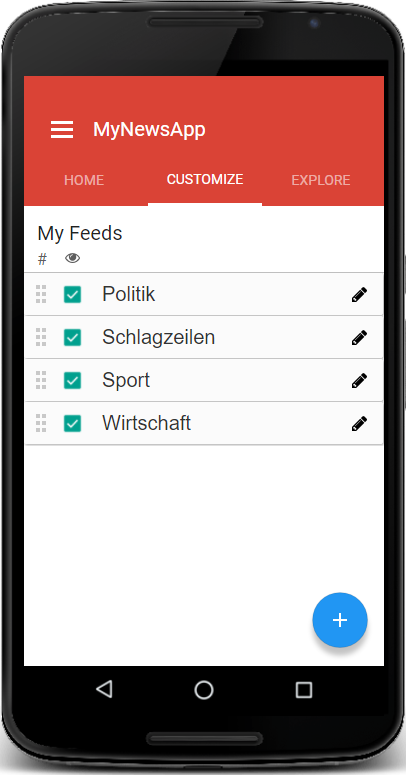
\includegraphics[width=0.4\textwidth]{screenshot 02}
  \caption{\enquote{Customize} Ansicht der MyNewsApp}
  \label{fig:screenshot-02}
\end{wrapfigure}

Die größten Änderungen hat der Menüpunkt Customize erfahren. Man erhält eine Übersicht aller Feeds, mit der Möglichkeit diese für den Homescreen anzupassen. Jeder Listeneintrag ist per Drag-and-Drop verschiebbar und kann unsichtbar geschalten werden. Durch kleine Piktogramme in der Kopfzeile der Liste werden diese Funktionen erklärt. Drückt man auf den Stift, so wird man direkt in die Bearbeitung des Feeds geschickt. Dabei ändert sich der Titel in der Menüleiste entsprechend um anzuzeigen, wo sich der Benutzer gerade befindet, falls nicht sicher ist wo genau er gedrückt hat oder falls er nach App-switchen nicht mehr genau weiß wo er war.

\clearpage

\begin{wrapfigure}{R}{0.45\textwidth}
  \centering
  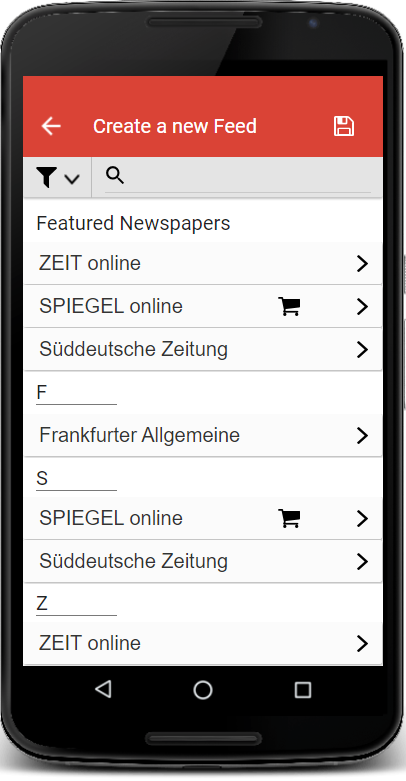
\includegraphics[width=0.4\textwidth]{screenshot 03}
  \caption{\enquote{Create a Feed} Ansicht der MyNewsApp}
  \label{fig:screenshot-03}
\end{wrapfigure}

Bei der Überarbeitung des Menüs zur Erstellung neuer Feeds wurde ein starker Fokus darauf gelegt, die Erstauswahl übersichtlicher zu gestalten. Auf dem Screen sieht man jetzt im ersten Schritt nur eine Auswahl aller verfügbaren Nachrichtenquellen in alphabetischer Reihenfolge. Eine kurze Featured-Sektion hilft dem Benutzer bei der Auswahl. Durch eine Suche und einen Filter für Kategorien lässt sich die Auswahl einschränken. Ist eine Auswahl getroffen, können im zweiten Schritt die Kategorien per Checkbox ausgewählt werden. Um nicht die Übersicht über ausgewählte Nachrichtenquellen zu verlieren, wird bei dem entsprechenden Titel im Obermenü ein Haken gesetzt, sobald man eine Kategorie in dieser Nachrichtenquelle ausgewählt hat. Um den Feed zu speichern, haben wir ein Disketten-Piktogramm, an dem für Android typischen Ort, eingeführt.

\clearpage

\begin{wrapfigure}{L}{0.45\textwidth}
  \centering
  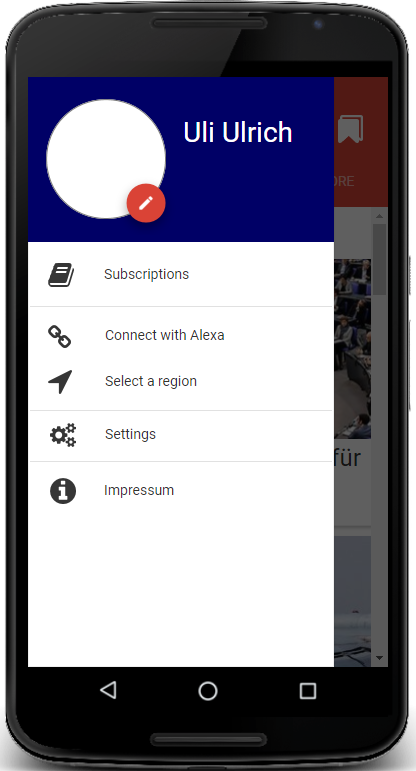
\includegraphics[width=0.4\textwidth]{screenshot 04}
  \caption{\enquote{User} Ansicht der MyNewsApp}
  \label{fig:screenshot-04}
\end{wrapfigure}

In das Burgermenü haben wir, um auch die neuesten Technologien einzubinden, die Option \enquote{Connect with Alexa} hinzugefügt. Digitale Assistenten werden erlangen zunehmend an Bedeutung, wie auch Beliebtheit, sodass dies nicht versäumt werden sollte. Denkbar wäre zum Beispiel, sich Nachrichten vorlesen zu lassen. Natürlich konnten wir die Funktionalität an sich nicht implementieren, aber mit dem Eintrag im Burgermenü sollte gezeigt werden, dass wir auch daran gedacht haben.

Aufgrund der Tatsache, dass wir bei unserer App keine Formulare oder ähnliche Inputs haben, war es nicht nötig, sich Gedanken über sinnvolle Default-Werte zu machen. Dies wäre aber auf jeden Fall zu beachten gewesen, hätte man zum Beispiel eine Registrierungsseite gehabt, bei der man das Herkunftsland auswählen muss. Beim Regionenfilter für Feeds ist es hingegen sinnvoll, den Standort des Nutzers per GPS zu bestimmen und so die Region vor- auszuwählen. Aber auch hier waren uns Grenzen durch Axure gesetzt, sodass wir dies nur durch entsprechende Schaltflächen andeuten konnten.

Im Menüpunkt Explore wurde, analog zu den neuen Piktogrammen in der Menüleiste von anderen Screens, der gewünschte zusätzliche Button zum Hinzufügen von Inhalten implementiert. Dieser ändert sich bei zahlungspflichtigen Inhalten, um ein Einkaufswagen-Piktogramm anzuzeigen. Zahlungspflichtige Inhalte sind außerdem beim Durchstöbern direkt im Titel durch ein Geldschein-Piktogramm erkennbar.

Beim Login wollten wir beachten, dass dieser einerseits schnell gehen muss, andererseits aber auch die typischen Loginmöglichkeiten über zum Beispiel einen Google-Account ermöglicht. Wir haben uns dazu entschieden, dass eine implizite Verbindung mit dem Google-Account hergestellt werden würde, wir also keinen Login-Screen implementieren. Einkäufe laufen dann einfach über das für den Benutzer bekannte System von In-App-Käufen. Würde man die App aber tatsächlich veröffentlichen, sollte man dem Nutzer dennoch die Wahl lassen, wie er sich einloggen möchte.

\clearpage

\begin{wrapfigure}{L}{0.45\textwidth}
  \centering
  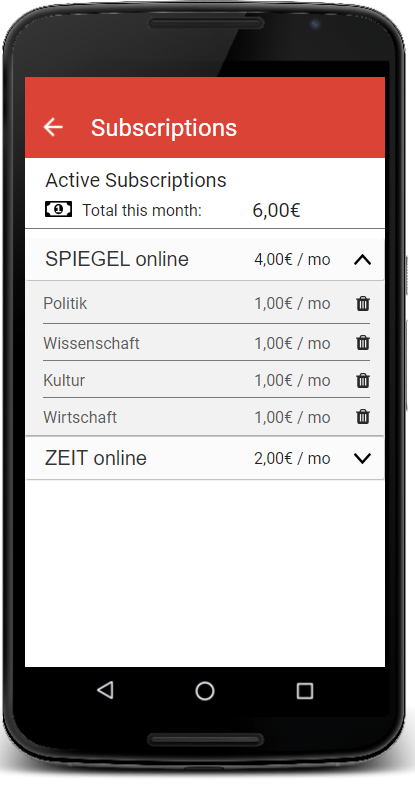
\includegraphics[width=0.4\textwidth]{screenshot 05}
  \caption{\enquote{Subscriptions} Ansicht der MyNewsApp}
  \label{fig:screenshot-05}
\end{wrapfigure}

Eine Möglichkeit zur Personalisierung eines Nutzerprofils darf jedoch in einer modernen App nicht fehlen, wurde aber nur angedeutet, da dies für die App kaum wirklichen Nutzen bietet.

Um Abonnements zu verwalten, haben wir einen komplett neuen Screen entworfen. Eine ausklappbare Liste aller aktiven Abonnements soll mehr Übersicht schaffen. Am Anfang der Liste erhält der Benutzer direkt die Summe für die nächste Abrechnung angezeigt. Dies wird dann zuerst per Nachrichtenquelle und dann noch per abonnierten Inhalt runtergebrochen. Mit dem Mülleimer-Piktogramm kann man den Eintrag direkt löschen. Da dies ohne zusätzliche Abfrage schnell zu Fehlern führen könnte, lässt sich diese Aktion mit Hilfe der Undo-Funktion sofort rückgängig machen. Diese Undo-Funktionalität wurde auch an anderen entscheidenden Stellen (z.b. beim Kauf von neuen Inhalten) eingebaut.

    % !TeX encoding=utf8
% !TeX spellcheck=de-DE
% !TeX root=../UID_Project_Documentation.tex

\section{Ausblick}

Mit der Erstellung eines zweiten Prototypen befinden wir uns nun in der zweiten Iteration des Projektes bei der Prototyping-Phase. Nun müsste zumindest noch einmal ein User Test erfolgen, um entweder festzustellen, dass die App ausreichend ausgereift ist, um sie zu veröffentlichen, oder dass noch weitere Verbesserungsmaßnahmen abgeleitet werden müssen, sodass noch ein oder gar mehrere Iterationszyklen durchlaufen werden sollten.

Ist die App dann ausreichend ausgereift designed, hängen die nächsten Schritte davon ab, welches Vorgehensmodell gewählt wurde. Beim Wasserfallmodell wäre nun die Implementation der App, also die tatsächliche Umsetzung, an der Reihe. Wurde eine agile Vorgehensweise gewählt, wäre die tatsächliche Entwicklung der App hingegen parallel zum Designen der UI der App verlaufen, sodass man nun schon ein releasebares Produkt hätte.

Wäre unsere Gruppe daran interessiert, die App wirklich umzusetzen und zu veröffentlichen, wäre es uns auf jeden Fall möglich gewesen, an die aus dieser Projektarbeit gewonnen Artefakte, Erkenntnisse, wie auch Ideen anzuknüpfen, um so mit einem großen Vorsprung in die \enquote{reale Welt} zu starten. Allerdings fürchten wir, dass die Konkurrenz durch große Anbieter viel zu groß ist, sodass es sehr schwer wäre, sich am Markt zu etablieren. Zudem ist auch der Aufwandsfaktor bei der Gründung eines Unternehmens enorm groß, sodass sich dies nur schwer mit dem Studium verbinden ließe. Als letzter Grund wäre noch zu nennen, dass wir alle bereits bei Unternehmen angestellt sind, die hochgradige Zukunftsperspektiven versprechen, sodass wir uns dazu entschieden haben, uns lieber auf eine Karriere in diesen Unternehmen zu konzentrieren, als im jungen Alter bereits selbst Unternehmensgründer zu werden.



\end{document}
